\chapter{Первая производная}
\label{chap:first-order}
\section{Касательная плоскость}

\begin{thm}{Определение}\label{def:tangent-vector}
Пусть $\Sigma$ --- гладкая поверхность.
Вектор $\vec w$ называется \index{касательный вектор}\emph{касательным} к $\Sigma$ в точке $p$ если найдётся кривая $\gamma$ на $\Sigma$ с вектором скорости $\vec w$ в точке $p$;
то есть $p=\gamma(t)$ и $\vec w=\gamma'(t)$ для некоторого~$t$.
\end{thm}

\begin{thm}{Предложение и определение}\label{def:tangent-plane}
Пусть $p$ --- точка на гладкой поверхности $\Sigma$.
Тогда множество касательных векторов к $\Sigma$ в точке $p$ образует плоскость;
эта плоскость называется \index{касательная!плоскость}\emph{касательной плоскостью} к $\Sigma$ в точке~$p$.

Более того, если $s\:U\to \Sigma$ --- локальная карта и $p=s(u_0,v_0)$, то 
касательная плоскость к $\Sigma$ в точке $p$ натянута на вектора $s_u(u_0,v_0)$ и $s_v(u_0,v_0)$.
\end{thm}

Касательная плоскость к $\Sigma$ в точке $p$ обозначается как $\T_p$ или $\T_p\Sigma$.
Эту плоскость можно рассматривать как линейное подпространство $\mathbb{R}^3$ или как параллельную плоскость, проходящую через~$p$;
последнюю можно называть \index{касательная плоскость}\emph{аффинной касательной плоскостью}.
Она даёт наилучшее приближение плоскостью окрестности $p$ в $\Sigma$.
Точнее, 
она имеет \index{порядок касания}\emph{первый порядок касания} с $\Sigma$ в точке $p$;
то есть $\rho(q)\z=o(|p\z-q|)$, где $q\in \Sigma$, а $\rho(q)$ обозначает расстояние от $q$ до $\T_p$.

Выбор касательного вектора $\vec v_p$ при каждой точке $p$ поверхности $\Sigma$ называется \emph{полем касательных векторов}, если $\vec v_p$ гладко зависит от $p$;
то есть в любой карте $s$ поле записывается как
\[\vec v_{s(u,v)}=a(u,v)\cdot s_u+b(u,v)\cdot s_v,\]
где $a$ и $b$ --- гладкие функции, определённые в области $s$.

\parbf{Доказательство.}
Выберем карту $s$ при~$p$.
Предположим, что гладкая кривая $\gamma$ начинается в~$p$.
Можно считать, что $\gamma$ накрыта картой;
в частности, 
\[\gamma(t)=s(u(t),v(t)).\]
для гладких функций $t\mapsto u(t)$ и $t\mapsto v(t)$.
По правилу дифференцирования сложной функции, 
\[\gamma'=s_u\cdot u'+ s_v\cdot v'.\]
В частности, $\gamma'$ является линейной комбинацией $s_u$ и $s_v$.

Поскольку гладкие функции $t\mapsto u(t)$ и $t\mapsto v(t)$ можно было выбрать произвольно, любая линейная комбинация $s_u$ и $s_v$ является касательным вектором в~$p$. 
\qeds

\begin{thm}{Упражнение}\label{ex:tangent-normal}
Поверхность $\Sigma$ задана как компонента связности множества уровня $f(x,y,z)=0$ гладкой функци $f:\mathbb{R}^3\to\mathbb{R}$ с регулярным значением $0$.
Покажите, что касательная плоскость $\T_p\Sigma$ перпендикулярна градиенту $\nabla_pf$ в любой точке $p\in\Sigma$.
\end{thm}

{\sloppy

\begin{thm}{Упражнение}\label{ex:vertical-tangent}
Пусть $\Sigma$ --- гладкая поверхность в $\mathbb{R}^3$, и $p\in\Sigma$.
Покажите, что окрестность $p$ в $\Sigma$ является графиком $z=f(x,y)$ гладкой функции $f$, определённой на открытом подмножестве в плоскости $(x,y)$, тогда и только тогда, когда касательная плоскость $\T_p$ не является {}\emph{вертикальной}; то есть если $\T_p$ не перпендикулярна горизонтальной плоскости.
\end{thm}

}

\begin{thm}{Упражнение}\label{ex:tangent-single-point}
Покажите, что если гладкая поверхность $\Sigma$ пересекает плоскость $\Pi$ в единственной точке $p$, то $\Pi$ является касательной к $\Sigma$ в~$p$.
\end{thm}

\section{Производная по направлению}\label{sec:dirder}

В этом разделе мы расширим определение производной по направлению на гладкие функции, определённые на гладких поверхностях.
Сначала вспомним стандартное определение для плоскости.

Даны точка $p\in \mathbb{R}^2$, вектор $\vec w\in \mathbb{R}^2$ и функция $f\:\mathbb{R}^2\to\mathbb{R}$.
Рассмотрим функцию
$h(t)=f(p+t\cdot\vec w)$.
Тогда производная по направлению функции $f$ в точке $p$ вдоль $\vec w$ определяется как \index{10d@$D_{\vec{w}}f$ (производная по направлению)}
\[D_{\vec w}f(p)\df h'(0).\]

Напомним, что функция $f\: \Sigma \to \mathbb{R}$ называется гладкой, если для любой карты $s\: U \to \Sigma$ композиция $f \circ s$ --- гладкая функция.

\begin{thm}{Предложение и определение}\label{def:directional-derivative}
Пусть $f$ --- гладкая функция, определённая на гладкой поверхности $\Sigma$.
Предположим, что $\gamma$ --- гладкая кривая в $\Sigma$, которая выходит из $p$ с вектором скорости $\vec{w}\in \T_p$;
то есть $\gamma(0)=p$ и $\gamma'(0)=\vec{w}$.
Тогда производная $(f\circ\gamma)'(0)$
зависит только от $f$, $p$ и $\vec{w}$;
она называется \index{производная по направлению}\emph{производной по направлению} функции $f$ вдоль $\vec{w}$ в точке $p$
и обозначается как
\[D_{\vec{w}}f,\quad D_{\vec{w}}f(p), \quad\text{или}\quad D_{\vec{w}}f(p)_\Sigma\] 
--- позволяется опускать $p$ и $\Sigma$, если всё ясно из контекста.

Более того, если $(u,v)\mapsto s(u,v)$ --- локальная карта, и $\vec{w}=a\cdot s_u \z+b\cdot s_v$ в точке $p$, то 
\[D_{\vec{w}}f=a\cdot (f\circ s)_u+b\cdot (f\circ s)_v.\]

\end{thm}

Если поверхность $\Sigma$ является плоскостью, то определение согласуется со стандартным.
Действительно, в этом случае $\gamma(t)=p+\vec w\cdot t$ является кривой в $\Sigma$, которая начинается в $p$ с вектором скорости~$\vec{w}$.
Однако, в общем случае точка $p+\vec w\cdot t$ не обязана лежать на поверхности,
и тогда значение $f(p+\vec w\cdot t)$ не определено.
В этом случае стандартное определение не работает.

\parbf{Доказательство.}
Не умаляя общности, можно предположить, что $p\z=s(0,0)$ и кривая $\gamma$ покрыта картой $s$.
В этом случае 
\[\gamma(t)=s(u(t),v(t))\]
для гладких функций $u,v$, определённых в окрестности точки $0$, таких что 
$u(0)\z=v(0)\z=0$.

По правилу дифференцирования сложной функции,
\begin{align*}
\gamma'(0)&=u'(0)\cdot s_u+v'(0)\cdot s_v
\end{align*}
в точке $(0,0)$.
Поскольку $\vec{w}=\gamma'(0)$ и векторы $s_u$, $s_v$ линейно независимы, мы получаем, что $a=u'(0)$ и $b=v'(0)$.

Применяя то же правило, получаем 
\[
(f\circ\gamma)'(0)=a\cdot (f\circ s)_u+b\cdot (f\circ s)_v.
\eqlbl{eq:f-gamma}
\]
в точке $(0,0)$.

Левая часть в \ref{eq:f-gamma} не зависит от выбора карты $s$, а правая зависит только от $p$, $\vec w$, $f$ и~$s$. 
Следовательно, $(f\circ\gamma)'(0)$ зависит только от $p$, $\vec w$ и~$f$.

Последнее утверждение следует из \ref{eq:f-gamma}.
\qeds


\begin{thm}{Продвинутое упражнение}\label{ex:lin-ind-chart}
Пусть $\vec x$ и $\vec y$ --- это векторные поля на гладкой поверхности $\Sigma$.
Предположим, что $\vec x_p$ и $\vec y_p$ линейно независимы в некоторой точке $p\in \Sigma$.
Постройте такие две функции $u$ и $v$ в окрестности точки $p$, что 
\begin{align*}
D_{\vec x} u&>0,
&
D_{\vec y} u&=0,
&
D_{\vec x} v&=0,
&
D_{\vec y} v&>0.
\end{align*}

Постройте карту на $\Sigma$ при $p$ с полями $\vec x$ и $\vec y$ касательными к координатным линиям.
\end{thm}

\section{Касательные векторы как функционалы}

В этом разделе даётся более концептуальное определение касательных векторов.
Мы не будем им пользоваться, но лучше о нём знать.

Касательный вектор $\vec w\in \T_p$ к гладкой поверхности $\Sigma$ 
определяет линейный функционал%
\footnote{Термин \emph{функционал} используется для функций, которые принимают функцию в качестве аргумента и возвращают число.} $D_{\vec w}$;
он заглатывает гладкую функцию $\phi$ на $\Sigma$, и выплёвывает  производную по направлению $D_{\vec w}\phi$.
Обратите внимание, что $D$ подчиняется правилу произведения, то есть
\[D_{\vec w}(\phi\cdot\psi)=(D_{\vec w}\phi)\cdot \psi(p)+\phi(p)\cdot(D_{\vec w}\psi).
\eqlbl{eq:tangent-functional}\]

Нетрудно показать, что касательный вектор $\vec w$ полностью определяется функционалом $D_{\vec w}$.
Более того, касательные векторы в точке $p$ могут \textit{определяться} как линейные функционалы на пространстве гладких функций, которые удовлетворяют тождеству \ref{eq:tangent-functional}.

Иначе говоря, тождество \ref{eq:tangent-functional} улавливает всё о касательных векторах.
Этот подход удобен в доказательствах, хотя он и не самый наглядный. 
Например, \ref{def:directional-derivative} превращается в тавтологию.

\section{Дифференциал}\label{sec:differential}

Любое гладкое отображение $s$ из поверхности $\Sigma_0$ в $\mathbb{R}^3$ можно описать его координатными функциями 
$s(p)=(x(p),y(p),z(p))$. 
Его производная по направлению, определяется покоординатно, то есть
\[D_{\vec{w}} s\df(D_{\vec{w}}x,D_{\vec{w}}y,D_{\vec{w}}z).\]

Предположим, что $s$ отображает одну гладкую поверхность $\Sigma_0$ в другую $\Sigma_1$.
Пусть $p_0\in \Sigma_0$ и $p_1=s(p_0)$.
Выберем такую кривую $\gamma_0$ на $\Sigma_0$, что $\gamma_0(0)=p_0$ и $\gamma_0'(0)=\vec w$.
Тогда $\gamma_1= s\circ \gamma_0$ --- гладкая кривая на~$\Sigma_1$. 
По определению производной по направлению, $D_{\vec w} s=\gamma_1'(0)$, и, значит, $D_{\vec w} s\in \T_{p_1}\Sigma_1$ для любого $\vec w\in \T_{p_0}$.

Из \ref{def:directional-derivative} вытекает, что
$\vec w \mapsto D_{\vec w} s$ определяет линейное отображение $\T_{p_0}\Sigma_0\z\to \T_{ p_1}\Sigma_1$;
то есть
\[D_{c\cdot \vec w} s=c\cdot D_{\vec w} s
\quad\text{и}\quad D_{\vec v+ \vec w} s=D_{\vec v} s+ D_{\vec w} s\]
для любых $c\in\mathbb{R}$ и $\vec v, \vec w\in\T_{p_0}$.
Отображение $d_{p_0} s\:\T_{p_0}\Sigma_0\z\to \T_{ p_1}\Sigma_1$, определяемое как
\[d_{p_0} s\:\vec w \mapsto D_{\vec w} s\]
называется \index{дифференциал}\emph{дифференциалом} $s$ при~$p_0$.


Дифференциал $d_{p_0} s$ описывается $2{\times}2$-матрицей $M$ в ортонормированных базисах $\T_{p_0}\Sigma_0$ и $\T_{p_1}\Sigma_1$.
Определим \index{якобиан}\emph{якобиан} $s$ при $p_0$ как $\jac_{p_0} s=|\det M|$; он  
не зависит от выбора ортонормированных базисов в $\T_{p_0}\Sigma_0$ и $\T_{p_1}\Sigma_1$.%
\label{page:|L|}\index{10d@$d_p f$ (дифференциал)}%
\footnote{Про $\jac_{p_0} s$ можно думать более геометрически:
если $R_0$ --- область в $\T_{p_0}$ и $R_1=(d_{p_0} s)(R_0)$ её образ, то
\[\area R_1=\jac_{p_0} s \cdot \area R_0.\]
Это равенство пригодится в определении площади поверхности.}

Если где $r\:\Sigma_1\to\Sigma_2$ --- ещё одно гладкое отображение между гладкими поверхностями $\Sigma_1$ и $\Sigma_2$, то
\[d_{p_0}( r\circ s)=d_{p_1} r \circ d_{p_0} s;\]
отсюда
\[\jac_{p_0}( r\circ s)
=
\jac_{p_1} r\cdot\jac_{p_0} s .\eqlbl{eq:jac-composition}\]

Приведённые выше построения применимы к карте $s$;
в этом случае поверхность $\Sigma_0$ является открытой областью в $\mathbb{R}^2$.
Тогда значение $\jac_{p_0} s$ можно найти с помощью формул
\begin{align*}
\jac s
&=|s_v\times s_u|=
\\
&=\sqrt{\langle s_u, s_u\rangle\cdot\langle s_v, s_v\rangle -\langle s_u, s_v\rangle^2}=
\\
&=\sqrt{\det[(\Jac s)^\top\cdot \Jac s ]},
\end{align*}
где $\Jac s$ обозначает матрицу Якоби $s$; см.~\ref{sec:Multivariable calculus}.

\section{Интеграл и площадь}

Пусть $\Sigma$ --- гладкая поверхность, и $h\:\Sigma\to\mathbb{R}$ --- гладкая функция.
Определим интеграл $h$ по борелеву множеству $R\subset \Sigma$;
чаще всего это определение будет применяться к поверхностям с границей.

Напомним, что якобиан $\jac_ps$ определён в предыдущем разделе.
Допустим, что существует карта $(u,v)\mapsto s(u,v)$ для $\Sigma$, определённая на открытом множестве $U\subset\mathbb{R}^2$, такая что $R\subset s(U)$.
В этом случае, определим
\[\iint_R h\df \iint_{s^{-1}(R)} h\circ s(u,v)\cdot \jac_{(u,v)}s \cdot du\cdot dv.\eqlbl{eq:area-def}\]

По правилу замены переменной (\ref{thm:mult-substitution}), правая часть в \ref{eq:area-def} не зависит от выбора~$s$.
То есть, если $s_1\:U_1\to \Sigma$ --- другая карта, такая что $s_1(U_1)\supset R$, то 
\[\iint_{s^{-1}(R)} h\circ s(u,v)\cdot \jac_{(u,v)}s \cdot du\cdot dv=\iint_{s_1^{-1}(R)} h\circ s_1(u,v)\cdot \jac_{(u,v)}s_1 \cdot du\cdot dv.\]
Другими словами, равенство \ref{eq:area-def} можно использовать как определение левой части.

В общем случае, область $R$ можно разбить на счётное число областей $R_1, R_2 \dots$, так что каждая $R_i$ лежит в образе карты
и определить интеграл по $R$ как сумму
\[\iint_Rh
\df
\iint_{R_1}h+\iint_{R_2}h+\dots\]
В случае, если $R$ компактно или же $h \geq 0$, легко проверить, что значение $\iint_Rh$ не зависит от выбора такого разбиения.


Площадь области $R$ на гладкой поверхности $\Sigma$ определяется как интеграл
\[\area R=\iint_R 1.\]

Следующее предложение даёт правило замены переменной для интеграла по поверхности.

\begin{thm}{Формула площади}\label{prop:surface-integral}
Пусть $s\:\Sigma_0\to \Sigma_1$ --- диффеоморфизм между гладкими поверхностями.
Рассмотрим область $R\subset \Sigma_0$ и гладкую функцию $f\:\Sigma_1\to\mathbb{R}$.
Предположим, что область $R$ компактна или же функция $f$ неотрицательна.
Тогда 
\[\iint_R (f\circ s)\cdot \jac s=\int_{s(R)}f.\]
В частности, при $f\equiv 1$, получаем
\[\iint_R \jac s=\area [s(R)].\]
\end{thm}

\parbf{Доказательство.}
Следует из \ref{eq:jac-composition} и определения интеграла по поверхности.
\qeds


Пусть $\Sigma_1$ и $\Sigma_2$ --- две гладкие поверхности.
Отображение $f\:\Sigma_1\z\to \Sigma_2$ называется \index{нерастягивающее отображение}\emph{нерастягивающим}, если для любой кривой $\gamma$ на $\Sigma$ выполняется $\length\gamma\ge \length (f\circ\gamma)$. 
Следующая теорема предоставляет более естественное определение площади.
Несмотря на интуитивную формулировку, доказательство выходит далеко за рамки нашей книжки;
оно основано на обобщении формулы площади для липшицевых отображений \cite[3.2.3]{federer}.


\begin{thm}{Теорема}\label{thm:area-axioms}
{\sloppy
Функционал площади удовлетворяет следующим свойствам:

}

\begin{subthm}{thm:area-axioms:aditivity}
Сигма-аддитивность: 
Пусть $R_1,R_2,\dots$ --- последовательность непересекающихся борелевских множеств на гладкой поверхности.
Тогда 
\[\area (R_1\cup R_2\cup \dots)=\area R_1+\area R_2+{}\dots\]
\end{subthm}

{\sloppy

\begin{subthm}{thm:area-axioms:monotonicity}
Монотонность:
Пусть $f\:\Sigma_1\to \Sigma_2$ --- нерастягивающее отображение между двумя гладкими поверхностями.
Предположим, что $R_1\subset \Sigma_1$ и $R_2\subset \Sigma_2$ --- такие борелевские множества, что $f(R_1)\supset R_2$.
Тогда 
\[\area R_1\ge \area R_2.\]
\end{subthm}

}

\begin{subthm}{thm:area-axioms:unit}
Единичный квадрат имеет единичную площадь. 
\end{subthm}

Более того, функционал площади однозначно определяется этими свойствами на всех борелевских множествах.
\end{thm}

\parit{Замечание.}
Понятия площади поверхности и длину кривой схожи.
Однако, длина определялась, используя другую идею (через верхнюю грань длин вписанных ломаных).
Известно, что аналогичное определение не работает даже для очень простых поверхностей.
Это видно из классического примера --- так называемого \textit{сапога Шварца}.
Этот пример и различные подходы к понятию площади обсуждаются в популярной статье Владимира Дубровского~\cite{dubrovsky}.


 \section{Вектор нормали и ориентация}
 
Единичный вектор, перпендикулярный $\T_p$, будет обычно обозначается как $\Norm(p)$;
он однозначно определён с точностью до знака.\index{10nu@$\Norm$ (поле нормалей)}

Поверхность $\Sigma$ называется \index{ориентированная поверхность}\emph{ориентированной}, если она снабжена полем  \index{нормаль}\index{поле нормалей}\emph{нормалей} $\Norm$;
то есть таким непрерывным отображением $p\mapsto \Norm(p)$, что $\Norm(p)\perp\T_p$ и $|\Norm(p)|=1$ для любого~$p$.
Выбор поля $\Norm$ называется {}\emph{ориентацией}~$\Sigma$.
Поверхность $\Sigma$ называется {}\emph{ориентируемой}, если её можно ориентировать.
Каждая ориентируемая поверхность допускает две ориентации: $\Norm$ и $-\Norm$.

Пусть $\Sigma$ --- гладкая ориентированная поверхность и $\Norm$ --- её поле нормалей.
Отображение $\Norm\:\Sigma\to \mathbb{S}^2$, определяемое как $p\mapsto \Norm(p)$, называется \index{сферическое!отображение}\emph{сферическим} или \index{гауссово отображение}\emph{гауссовым}.

\begin{wrapfigure}{r}{42 mm}
\vskip-7mm
\centering
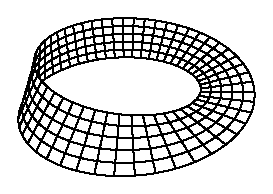
\includegraphics{asy/moebius}
\vskip-1mm
\end{wrapfigure}

Для поверхностей сферическое отображение играет ту же роль, что и касательная индикактриса для кривых.

Лента Мёбиуса, показанная на рисунке, даёт пример неориентируемой поверхности --- поле нормалей нельзя продолжить непрерывно вдоль средней линии ленты (при попытке обойти ленту вокруг нормаль меняет знак).

Каждая поверхность локально ориентируема.
Более того, каждая карта $s(u,v)$ допускает ориентацию 
\[\Norm=
\frac{s_u\times s_v}
{\left|s_u\times s_v\right|}.\]
Действительно, векторы $s_u$ и $s_v$ являются касательными векторами в точке $p$.
Значит, их векторное произведение перпендикулярно касательной плоскости,
и оно не обращается в ноль
и так как $s_u$ и $s_v$ линейно независимы.
Ясно, что отображение $(u,v)\mapsto \Norm(u,v)$ непрерывно.
Следовательно, $\Norm$ --- это поле единичных нормалей.

{\sloppy

\begin{thm}{Упражнение}\label{ex:const-normal}
Предположим, что гладкая поверхность $\Sigma$ имеет постоянное поле нормалей $\nu_0$.
Покажите, что $\Sigma$ лежит в плоскости, перпендикулярной к $\nu_0$.
\end{thm}

}

\begin{thm}{Упражнение}\label{ex:implicit-orientable}
Пусть $0$ --- регулярное значение гладкой функции
$h:\mathbb{R}^3\to\mathbb{R}$.
Покажите, что компонента связности множества уровня $h(x,y,z)=0$ есть ориентируемая поверхность.
\end{thm}

Напомним, что любая собственная поверхность $\Sigma$ без границы в евклидовом пространстве делит его на две связные компоненты (\ref{clm:proper-divides}).
Следовательно, мы можем выбрать поле единичных нормалей на $\Sigma$, которое указывает в одну из компонент дополнения; таким образом, мы получаем следующее.

\begin{thm}{Замечание}
Любая гладкая собственная поверхность без границы в евклидовом пространстве является ориентируемой.
\end{thm}

В частности, ленту Мёбиуса нельзя продолжить до собственной гладкой поверхности без границы.

\section{Сечения}

\begin{thm}{Лемма}\label{lem:reg-section}
Пусть $\Sigma$ --- гладкая поверхность, и $f\:\Sigma\to\mathbb{R}$ --- гладкая функция.
Для любой константы $r_0$ найдётся сколь угодно близкое $r$, такое что 
каждая компонента связности линии уровня $L_r=\set{x\in\Sigma}{f(x)=r}$ была бы гладкой кривой.
\end{thm}

\parbf{Доказательство.}
Поверхность $\Sigma$ можно покрыть счётным набором карт $s_i\:U_i\to \Sigma$.
При этом композиция $f\circ s_i$ является гладкой функцией для любого $i$.
По лемме Сарда (\ref{lem:sard}), почти всех $r\in \mathbb{R}$ являются регулярным значением каждой композиции $f\circ s_i$.

Зафиксируем такое значение $r$, достаточно близкое к $r_0$, и рассмотрим множество $L_r$, описываемое уравнением $f(x,y,z)=r$.
Любая точка в $L_r$ лежит в образе одной из карт.
Следовательно, эта точка имеет окрестность, которая является гладкой кривой;
отсюда результат.
\qeds

\begin{thm}{Продвинутое упражнение}\label{ex:plane-section}
Пусть $\Pi$ --- координатная плоскость $z=0$, и $A \subset \Pi$ --- любое замкнутое подмножество.
Постройте такую открытую гладкую поверхность $\Sigma$, что $\Sigma \cap \Pi = A$.
\end{thm}

Упражнение выше показывает, что сечения плоскостью гладкой поверхности можно сделать довольно противным.
Следствие ниже позволяет подсдвинуть плоскость, чтобы сечение стало вести себя приемлемо.

\begin{thm}{Следствие}
Пусть $\Sigma$ --- гладкая поверхность.
Тогда для любой плоскости $\Pi$ существует параллельная плоскость $\Pi^{*}$, лежащая сколь угодно близко к $\Pi$ и такая, что пересечение $\Sigma\cap\Pi^{*}$ есть объединение непересекающихся гладких кривых.
\end{thm}
